\chapter{Introducción}

\section{Contexto y motivación}

La movilidad urbana atraviesa una transformación profunda. El transporte es uno de los principales emisores de gases de efecto invernadero en Europa y, dentro de él, el tráfico rodado en las ciudades concentra buena parte de las emisiones y de la contaminación atmosférica que respiran los ciudadanos. Ante este problema, las administraciones han pasado de recomendar a obligar. La Agenda 2030 y los objetivos europeos de neutralidad climática marcan la dirección, y en España la Ley 7/2021, de 20 de mayo, de cambio climático y transición energética~\cite{BOELey7_2021} obliga a los municipios de más de \numprint{50000} habitantes a implantar \glspl{zbe}, que restringen la circulación de los vehículos más contaminantes en amplias áreas del centro urbano. En paralelo, los ayuntamientos elaboran planes de movilidad urbana sostenible que buscan reducir la dependencia del coche privado y desplazar los viajes hacia el transporte público y los modos activos.\newline

Este giro normativo convierte el reparto modal, es decir, la proporción de viajes que se realizan en cada modo de transporte, en una variable central de la política urbana. Peatonalizar una calle, ampliar una \gls{zbe}, modificar el trazado o la frecuencia de una línea de autobús o cambiar el precio del billete son decisiones que persiguen, en último término, alterar ese reparto en favor de modos más sostenibles. Sin embargo, son también decisiones costosas, difíciles de revertir y políticamente sensibles, pues afectan a la vida diaria de miles de personas y su aceptación depende de que se perciban como razonables y favorables para el ciudadano.\newline

Aquí surge la necesidad que motiva este trabajo. Quienes diseñan la red y legislan sobre movilidad (técnicos municipales, planificadores y responsables políticos) necesitan que sus políticas sean lo más acertadas y beneficiosas posible antes de aplicarlas, y para ello han de anticipar cómo reaccionarán los viajeros. ¿Cuántos usuarios dejarían de utilizar el coche para ir a trabajar si el precio de un billete de autobús urbano bajara un 20\%? ¿Y si una línea aumentara su frecuencia o cambiara su recorrido? ¿Qué efecto tendría encarecer el aparcamiento en el centro? Responder a estas preguntas por ensayo y error sobre la propia ciudad es inviable. Se requieren herramientas que permitan generar gemelos digitales de la ciudad y explorar estos escenarios \textit{what-if} de forma anticipada, comparando el efecto de cada medida sobre el comportamiento previsible de los viajeros.\newline

La confluencia de dos avances hace hoy posible construir ese tipo de herramienta. Por un lado, la disponibilidad de datos abiertos: la cartografía colaborativa de \acrlong{osm} y los feeds \acrshort{gtfs} de transporte público publicados por las administraciones permiten calcular tiempos y costes realistas de cualquier trayecto en cualquier modo. Por otro, la madurez de las técnicas de aprendizaje automático, que han demostrado mejorar la capacidad predictiva de los modelos clásicos de elección discreta a la hora de estimar qué modo de transporte elegirá un viajero en función de sus características y de las condiciones del viaje. Combinar ambos elementos en una aplicación interactiva y accesible es precisamente el hueco que este trabajo pretende cubrir.

\begin{figure}[htbp]
  \centering
  % \missingfigure{Imagen motivadora de movilidad urbana sostenible: señalización de una zona de bajas emisiones (ZBE) en una ciudad española, o composición de modos de transporte urbano (autobús, bicicleta, peatones) en un entorno urbano. Tamaño moderado (unos dos tercios del ancho de página).}
  % \caption{Movilidad urbana sostenible y zonas de bajas emisiones.}
  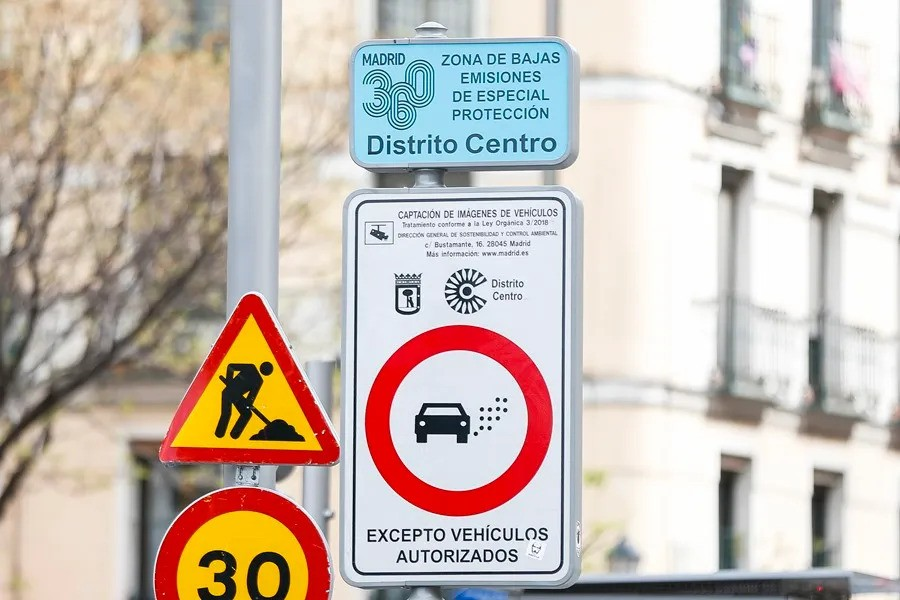
\includegraphics[width=0.72\textwidth]{figs/ZBE_Madrid_Obras.jpg}
  \caption{Señal de zona de bajas emisiones junto a una señal de obras en el centro de Madrid. Fuente: EFE/Víctor Casado.}
  \label{fig:motivacion}
\end{figure}

\newpage
En este trabajo de fin de máster se propone el desarrollo de un simulador web de movilidad urbana que, a partir de datos abiertos de la red de transporte público (paradas, líneas y horarios) y de una serie de atributos del viajero, permita simular cómo se comportarán los usuarios ante un escenario concreto y estimar cómo les afecta. El simulador integra modelos de aprendizaje automático para predecir la elección modal y servicios de enrutado que aportan los tiempos y costes reales de cada modo, y expone controles para modificar los parámetros del escenario. De este modo, ofrece a legisladores, gestores y diseñadores de la red y de las políticas de movilidad un entorno para ensayar escenarios \textit{what-if} y anticipar su impacto en el reparto modal antes de llevarlos a la práctica.

\section{Objetivos del TFM}

\subsection{Objetivo general}

Desarrollar un prototipo de simulador web de movilidad urbana que integre modelos de predicción basados en Machine Learning y servicios de enrutado, con el fin de analizar el impacto de distintas políticas de transporte en el reparto modal de los viajes y servir de apoyo a la planificación y la toma de decisiones en movilidad urbana.

\subsection{Objetivos específicos}

\begin{itemize}
    \item Entrenar y validar modelos de Machine Learning con datos de movilidad para predecir la elección modal de los usuarios en función de variables sociodemográficas, de tiempo y de coste.
    \item Integrar servicios de enrutado (\acrshort{osrm} y \acrshort{otp}) para obtener tiempos y costes realistas entre pares origen-destino en el entorno urbano.
    \item Desarrollar una aplicación web interactiva que permita definir viajes sobre un mapa, simular el comportamiento de los usuarios y visualizar resultados en un cuadro de mando.
    \item Implementar un módulo de análisis de escenarios \textit{what-if} para modificar parámetros de política (coste del coche, tarifas del transporte público, frecuencia de autobuses, etc.) y observar su efecto en el reparto modal.
    % \item Generar métricas de impacto (reparto modal, tiempo medio de viaje y estimación de emisiones de CO\textsubscript{2}) como apoyo a la toma de decisiones en movilidad urbana.
\end{itemize}

\subsection{Competencias trabajadas}

El desarrollo del TFM contribuye a las siguientes competencias del Máster:

\begin{itemize}
    \item \textbf{CP01}: Integrar tecnologías, aplicaciones, servicios y sistemas de la Ingeniería Informática en un contexto multidisciplinar.
    \item \textbf{CP05}: Aplicar métodos matemáticos, estadísticos y de inteligencia artificial para modelar y desarrollar sistemas inteligentes.
    \item \textbf{CP07}: Realizar un proyecto integral original de carácter profesional que sintetice las competencias adquiridas en el plan de estudios.
\end{itemize}

\section{Estructura del documento}

El resto de la memoria se organiza en los siguientes capítulos:
\begin{itemize}
  \item El \textbf{Capítulo~\ref{ch:estadoarte}} revisa el estado del arte y el marco tecnológico: los fundamentos del modelado de la elección modal, desde los modelos clásicos de elección discreta hasta las técnicas de aprendizaje automático, y las tecnologías de datos abiertos y enrutado en las que se apoya el simulador.
  \item El \textbf{Capítulo~\ref{ch:metodologia}} describe la metodología de trabajo, un proceso Scrum adaptado a un desarrollo unipersonal, junto con el histórico de sprints ejecutados y la retrospectiva del ciclo de desarrollo.
  \item El \textbf{Capítulo~\ref{ch:arquitectura}} presenta la arquitectura del sistema: los componentes que lo forman, su despliegue mediante contenedores y las principales decisiones de diseño.
  \item El \textbf{Capítulo~\ref{ch:implementacion}} detalla la implementación de cada componente (enrutado, transporte público, backend, frontend y modelos de elección modal) y los resultados obtenidos en el entrenamiento y la evaluación.
  \item El \textbf{Capítulo~\ref{ch:conclusiones}} recoge las conclusiones, revisando el cumplimiento de los objetivos, y plantea las líneas de trabajo futuro.
\end{itemize}

Al final del documento se incluyen los anexos, con el manual de despliegue, el detalle de los endpoints de la API y la configuración experimental para la reproducibilidad de los resultados.